\documentclass[10pt,a5paper,titlepage,oneside]{book}
%\documentclass{article} % Specifies the document class
%\usepackage[cp1251]{inputenc}


\usepackage[T1,T2A]{fontenc}
\usepackage[utf8]{inputenc}


%\usepackage[T1,T2A]{fontenc}
%\usepackage[cp1251]{inputenc}


\usepackage[intlimits,sumlimits]{amsmath}
\usepackage{amsmath}

\usepackage{enumerate,graphicx,dcolumn,amsthm}
\usepackage[english,ukrainian]{babel}
\usepackage{indentfirst}
\usepackage{caption}[2013/01/20]
%\captionsetup{labelsep=period,font=sf, labelfont=bf, format=plain, justification=centerlast, tablename=Таблиця}
\captionsetup{labelsep=period,font=sf, labelfont=bf, format=plain, justification=justified, tablename=Таблиця, tablewithin=none}

\usepackage{graphicx}
\graphicspath{{Fig/}}
\usepackage{floatflt}
\usepackage{wrapfig}
\usepackage{afterpage}

\usepackage{tabularx}
\renewcommand{\tabularxcolumn}[1]{m{#1}}
\usepackage{hhline}
\usepackage{multirow}
\usepackage{tabu}

\usepackage{longtable}
\usepackage{colortbl}
\definecolor{MyGray}{gray}{0.9}
\doublerulesepcolor[rgb]{1,1,1}

\usepackage{tikz}
\usetikzlibrary{calc}
\usepackage{wrapfig}

 \usepackage[left=20mm,right=15mm,top=15mm,bottom=16mm,bindingoffset=0mm,footskip=6mm,includefoot]{geometry}
\setlength{\parindent}{5mm}
\usepackage[hang,flushmargin]{footmisc}

\pagestyle{plain}



    \usepackage{enumitem}
    \makeatletter
        \AddEnumerateCounter{\asbuk}{\@asbuk}{м)}
    \makeatother
%    \setlist{nolistsep}
%  \setlist{itemindent=0cm,topsep=0cm,parsep=0cm,itemsep=0cm,labelindent=0cm}
   \setlist{nolistsep, topsep=0ex, leftmargin=1ex, itemindent=4ex}
%    \renewcommand{\labelitemi}{$\bullet$}
    \renewcommand{\labelenumi}{\arabic{enumi}.}
    \renewcommand{\labelenumii}{\asbuk{enumii})}



\numberwithin{equation}{part}


\makeatletter


\usepackage {titlesec}
\titleformat{\chapter}{\hyphenpenalty=10000\sf\Large\bfseries}{
\thechapter. }{0pt}{\Large}

\titlespacing*{\chapter}{0pt}{1.1\baselineskip}{\baselineskip}

\titleformat{\section}{\hyphenpenalty=10000\sf\large\bfseries}{
\thesection. }{0pt}{\large}

\makeatother



%\includeonly{
%%title,
%%acronyms,
%%vstup,
%Evolution,
%Swarm,
%Bio,
%Human,
%Physical,
%Math,
%Other,
%Hybrid,
%Multi
%}

\usepackage{pifont}
% Подключаемый Symbol-шрифт,
% Обеспечивает доступность семейства \verb|U/psy/m/n| под именем greek
\DeclareSymbolFont{greek}{U}{psy}{m}{n}
% Выбор команды переключения шрифта
\DeclareSymbolFontAlphabet{\gr}{greek}



\renewcommand{\theequation}{\thechapter.\arabic{equation}}

\usepackage{cite}
\bibliographystyle{utf8gost780u}
%\bibliographystyle{model1-num-names}
%\bibliographystyle{ieeetr}
%\bibliographystyle{acm}

\begin{document}           % End of preamble and beginning of text.

\renewcommand\bibname{Список використаних джерел}
\renewcommand{\tablename}{Табл.}

\setcounter{chapter}{1}
\setcounter{section}{1}

\section{Методи до визначення рухливості у кремнії}

Задача оцінки рухливості електронів $\mu_n$ та дірок $\mu_p$ у напівпровіднику
за певних умов є достатньо поширеною у різноманітних фізичних дослідженнях.
Один з варіантів її вирішення полягає у використанні загального підходу, згідно з яким
\begin{equation}\label{eqG}
  \mu=\frac{e\tau_p}{m_\sigma}\,,
\end{equation}
де
$e$ --- елементарний заряд,
$\tau_p$ --- середній час вільного пробігу носія заряду,
$m_\sigma$ --- ефективна маса електропровідності.

Час вільного пробігу обмежується розсіянням носіїв заряду, яке може бути викликане декількома причинами,
пов'язаними з порушеннями періодичності потенціалу.
Зокрема виділяють розсіяння на коливаннях ґратки (акустичних та оптичних фононах), заряджених та нейтральних домішках,
дислокаціях, границях зерен та інших неоднорідностях структури, поверхнях та межах розділу, інших носіях.
Кожен із цих механізмів має свою залежність від температури, рівня легування та розміру напівпровідникової структури
і може бути визначальним для величини рухливості за певних умов.
Проте найчастіше необхідно враховувати декілька можливих шляхів розсіяння носіїв заряду.
В такому випадку для оцінки рухливості використовується правило Маттісена:
\begin{equation}\label{eqM}
  \mu^{-1}=\sum_i \mu_i^{-1}\,,
\end{equation}
де
сумування відбувається за механізмами розсіяння,
$\mu_i$ --- рухливість носіїв за наявності лише $i$-го механізму розсіяння.
Для оцінки $\mu_i$ можна використовувати вирази, аналогічні формулі (\ref{eqG}), розрахувавши відповідний час вільного пробігу.

Для переважної більшості механізмів розсіяння вирази для оцінки рухливості відомі.
Так, при розсіянні на іонізованих домішках нерідко використовується вираз Brooks \& Herring \cite{Seeger2004}:
\begin{equation}\label{eqBH}
  \mu_\mathrm{I}=\frac{3,68\cdot10^{20}\text{см}^{-3}}{N_\mathrm{I}Z^2}\left(\frac{\varepsilon}{16}\right)^2\left(\frac{T}{100\,\mathrm{K}}\right)^{1,5}
  \frac{\left({m_0}/{m}\right)^{0,5}}{\left[\lg(1+\beta^2_\mathrm{BH})-\frac{0,434\beta^2_\mathrm{BH}}{1+\beta^2_\mathrm{BH}}\right]}\,,
\end{equation}
де
$N_\mathrm{I}$ --- концентрація домішок із зарядом $Ze$,
$\varepsilon$ --- діелектрична проникність напівпровідника,
$T$ --- температура,
$m$ ---ефективна маса носія,
$m_0$ --- маса вільного електрону,
а величина $\beta_\mathrm{BH}$ має вигляд
\begin{equation}\label{eqBH2}
  \beta_\mathrm{BH}=\left(\frac{\varepsilon}{16}\right)^{0,5} \frac{T}{100\,\mathrm{K}} \left(\frac{m}{m_0}\right)^{0,5}
  \left(\frac{2,08\cdot10^{18}\text{см}^{-3}}{n_c}\right)^{0,5}\,,
\end{equation}
$n_c$ --- концентрація носіїв заряду.
Іншим наближенням для такого випадку є формула Conwell \& Weisskopf \cite{Seeger2004}:
\begin{equation}\label{eqCW}
\begin{aligned}
    \mu_\mathrm{I} &=\frac{3,68\cdot10^{20}\text{см}^{-3}}{N_\mathrm{I}Z^2}\left(\frac{\varepsilon}{16}\right)^2\left(\frac{T}{100\,\mathrm{K}}\right)^{1,5}
  \frac{\left({m_0}/{m}\right)^{0,5}}{\lg\left(1+\beta^2_\mathrm{CW}\right)}\,, \\
   \beta_\mathrm{CW} &=\frac{1}{Z} \frac{\varepsilon}{16}\frac{T}{100\,\mathrm{K}}\left(\frac{2,35\cdot10^{19}\text{см}^{-3}}{N_\mathrm{I}}\right)^{1/3}\,.
\end{aligned}
\end{equation}

Для іншого механізму, розсіяння носій-носій застосовується підхід, розвинутий Fletcher \cite{Fletcher1957}:
\begin{equation}\label{eqFl}
  \mu_{cc}=\frac{\left(\frac{T}{T_{ref}^{Fl}}\right)^{3/2} F_1}{\left(np\right)^{1/2}\ln\left[1+\left(\frac{T}{T_{ref}^{Fl}}\right)^2\left(np\right)^{-1/3}F_2\right]}\,,
\end{equation}
де
$n$ та $p$ --- концентрації електронів та дірок, відповідно;
$T_{ref}^{Fl}$, $F_1$ та $F_2$ --- певні константи, які залежать від матеріалу.
Як показано в роботах \cite{Choo1972,Dorkel1981}, для кремнію доцільно застосовувати 
$T_{ref}^{Fl}=300$~K,
$F_1=1,04\cdot10^{21}$~см$^{-1}$В$^{-1}$с$^{-1}$,
$F_2=7,45\cdot10^{12}$~см$^2$ і тоді вираз (\ref{eqFl}) перетворюється на наступний
\begin{equation}\label{eqDorkel}
  \mu_{cc}=\frac{2\cdot10^{17}T^{3/2}}{\sqrt{n\,p}\ln\left[1+8,28\cdot10^8T^2\left(np\right)^{-1/3}\right]}\,.
\end{equation}

Проте в більшості випадків для більш-менш точного опису рухливості реального матеріалу необхідно враховувати значну кількість механізмів.
Як наслідок, більше поширення отримав підхід оцінки величини $\mu$ з використанням апроксимаційної функції, яка часто базується на результатах експериментальних вимірювань.
Як правило, для кожного матеріалу вигляд функції або наявні в ній коефіцієнти відрізняються.

Розглянемо декілька подібних підходів до опису рухливості носіїв заряду у монокристалічному кремнії, обмежуючись випадками об'ємного напівпровідника 
(без врахування впливу поверхні) та слабких полів.
Одним з перших подібних наближень був вираз, запропонований   Caughey \& Thomas \cite{Caughey1967}:
\begin{equation}\label{eqCT}
  \mu=\mu_\mathrm{min}+\frac{\mu_\mathrm{max}-\mu_\mathrm{min}}{1+(N/N_{ref})^\alpha}\,,
\end{equation}
де 
$N$ --- концентрація легантів, 
а значення констант для випадків, коли розглядаються рухливості електронів та дірок, наведені у Табл.~\ref{tblCT}.
Вираз насамперед призначений для оцінки залежності рухливості основних носіїв від концентрації легуючої домішки поблизу 300~K.
З іншого боку, формула (\ref{eqCT}) не дозволяє оцінити рухливості неосновних носіїв та не враховує температурну залежність $\mu$.


\begin{table}
\caption{Коефіцієнти для розрахунку рухливості відповідно до моделі Caughey--Thomas (\ref{eqCT})}
\label{tblCT}
\centering
\begin{tabular}{|l|c|c|c|c|}
\hline
\multirow{2}{*}{Тип носіїв} & \multicolumn{4}{c|}{Параметр} \\
\cline{2-5}
&$\mu_\mathrm{max}$, $\text{см}^2/(\text{B}\cdot\text{с})$&$\mu_\mathrm{min}$, $\text{см}^2/(\text{B}\cdot\text{с})$&$\alpha$&$N_{ref}$, см$^{-3}$ \rule{0pt}{13pt}\\
\hline
Електрони&1330&65&0,72&$8,5\cdot10^{16}$\\
Дірки&495&47,7&0,76&$6,3\cdot10^{16}$\\
\hline
\end{tabular}
\end{table}



\cite{Masetti1983}

\begin{equation}\label{eqMas}
\begin{aligned}
    \mu_n &=\mu_0+\frac{\mu_\mathrm{max}-\mu_0}{1+\left(\frac{n}{C_r}\right)^a}-\frac{\mu_1}{1+\left(\frac{C_s}{n}\right)^b}\,, \\
   \mu_p &=\mu_0\exp\left(-\frac{p_c}{p}\right)+\frac{\mu_\mathrm{max}}{1+\left(\frac{p}{C_r}\right)^a}-\frac{\mu_1}{1+\left(\frac{C_s}{p}\right)^b}\,.
\end{aligned}
\end{equation}


\begin{table}
\caption{Коефіцієнти для розрахунку рухливості відповідно до моделі Masetti (\ref{eqMas})}
\label{tblMas}
\centering
\begin{tabular}{|l|c|c|}
\hline
\multirow{2}{*}{Параметр} & \multicolumn{2}{c|}{Легант} \\
\cline{2-3}
&Фосфор&Бор\\
\hline
$\mu_0$, $\text{см}^2/(\text{B}\cdot\text{с})$&68,5&44,9\\
\hline
$\mu_\mathrm{max}$, $\text{см}^2/(\text{B}\cdot\text{с})$&1414&470,5\\
\hline
$\mu_0$, $\text{см}^2/(\text{B}\cdot\text{с})$&56,1&29,0\\
\hline
$C_r$, см$^{-3}$&$9,2\cdot10^{16}$&$2,23\cdot10^{17}$\\
\hline
$C_s$, см$^{-3}$&$3,41\cdot10^{20}$&$6,10\cdot10^{20}$\\
\hline
$a$&0,711&0,719\\
\hline
$b$&1,98&2,00\\
\hline
$p_c$, см$^{-3}$&---&$9,23\cdot10^{16}$\\
\hline
\end{tabular}
\end{table}


\cite{Arora1982}
\begin{equation}\label{eqArora}
  \mu=\mu_\mathrm{min}+\frac{\mu_0}{1+\left(\frac{N}{N_0}\right)^\alpha}
\end{equation}

\begin{equation}\label{eqArora2}
\begin{aligned}
    \mu_\mathrm{min} &=\mu_\mathrm{min}^{ref}\left(\frac{T}{T_{ref}}\right)^{\beta_1}\,, \\
   \mu_0 &=\mu_0^{ref}\left(\frac{T}{T_{ref}}\right)^{\beta_2}\,,\\
   N_0 &=N_0^{ref}\left(\frac{T}{T_{ref}}\right)^{\beta_3}\,,\\
   \alpha &=\alpha^{ref}\left(\frac{T}{T_{ref}}\right)^{\beta_4}\,.\
\end{aligned}
\end{equation}


неосновні електрони \cite{Swirhun1986}
неосновні дірки \cite{Alamo1985}



%Carrier mobility in a semiconductor is one of the most
%important parameters for the operation of electronic
%devices. Actually, the mobility measures the ability of
%free carriers (electrons or holes) to move in the material
%as it is subjected to an external electric field. The magni-
%tude of the mobility directly impacts on the device perform-
%ance since it determines the operation speed through the
%transit time across the device, the circuit operating fre-
%quency, or the sensitivity in magnetic sensors.

%THE ELECTRON tion of dopant concentration and temperature and hole mobilities in silicon as a func- are
%important parameters for device design and analysis.


%\begin{titlepage}
\begin{center}

{\small Київський національний університет  імені Тараса Шевченка}

{\small фізичний факультет}


\vspace*{2cm}
{\scshape\bfseries\Large О.Я.~ОЛІХ}

\vspace*{1cm}
{\scshape\bfseries\huge методи дослідження дефектів}

\vspace*{0.5cm}
методичний посібник для студентів фізичного факультету

\end{center}
%
%%\vspace*{1cm}
\begin{figure}[h]\center
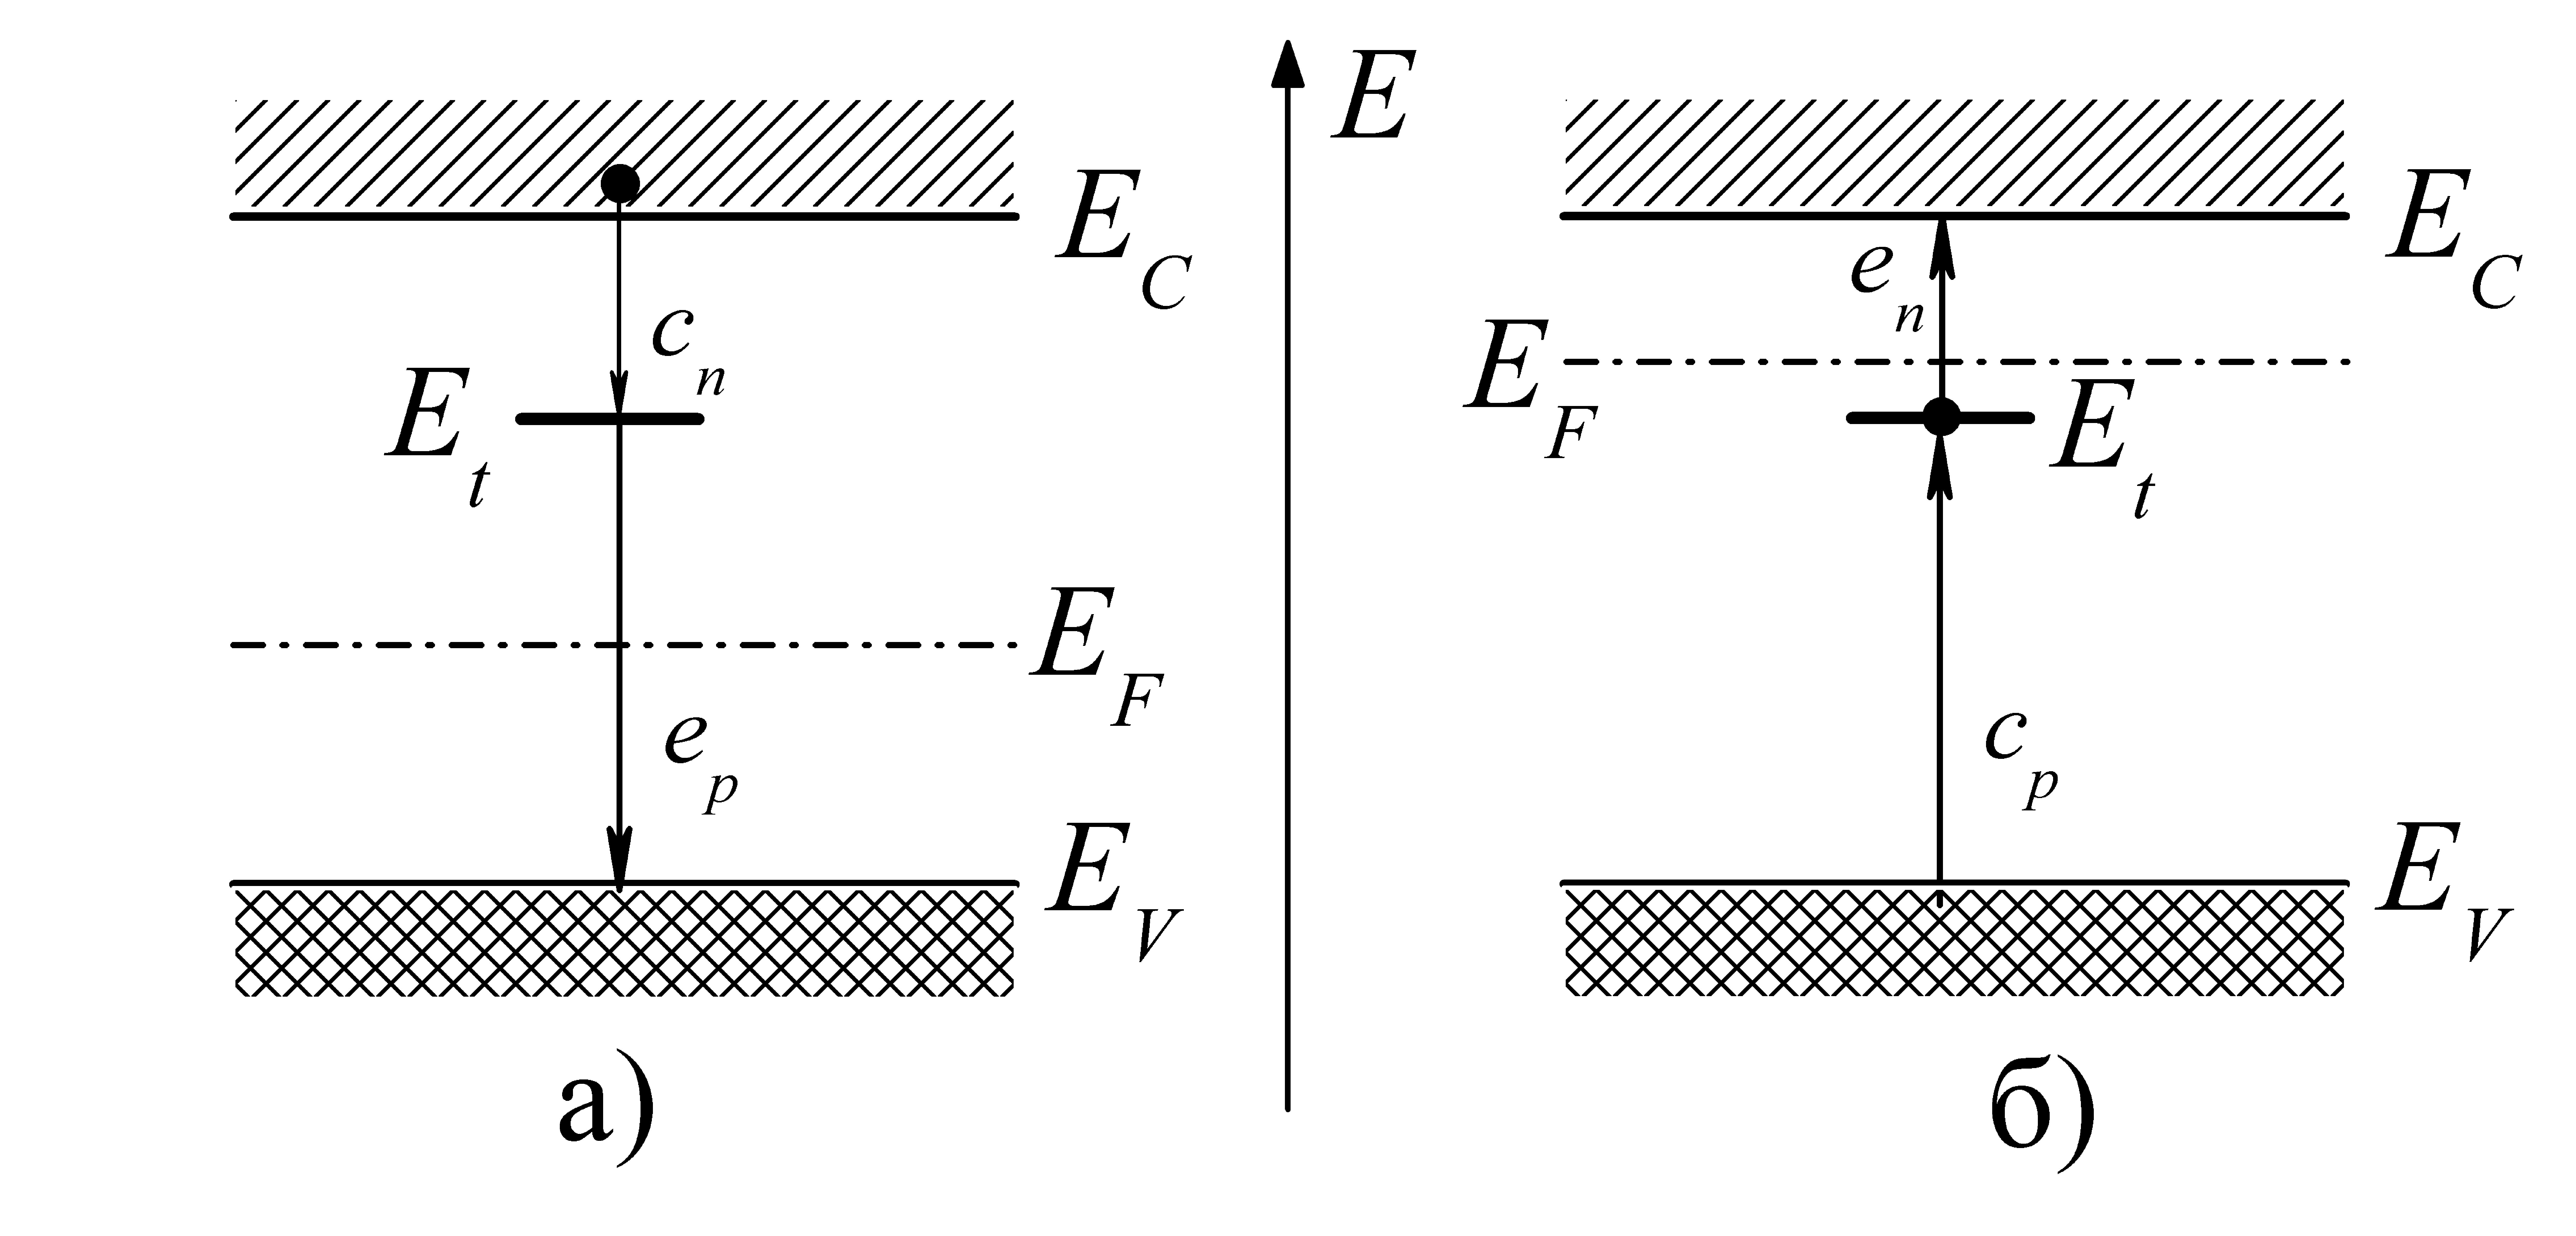
\includegraphics[width=0.4\textwidth]{Fig1_1}
\end{figure}
%
%
\begin{center}

{\scshape\bfseries Київ -- 2020}
\end{center}
\end{titlepage}
Б

УДК 004.7; 004.057.4.

\begin{center}

 \vspace{0.04\textheight}
 Рецензенти:
\end{center}
%\vspace{0.5cm}

\emph{С.В.~Кондратенко}, д-р. фіз.-мат. н., проф.

\emph{О.О.~Коротченков}, д-р. фіз.-мат. н., проф.

\vspace{1cm}
Рекомендовано до друку вченою радою фізичного факультету
Київського національного університету імені Тараса Шевченка
(протокол №10 від 18 квітня 2020 року)



\vspace{1cm}
\textbf{Оліх О.Я.}

Методи дослідження дефектів. Методичний посібник для студентів фізичного факультету. --- К.:2020.
%Іл.~236, табл.~51.

\vspace{1cm}
У посібнику розглянуто основні типи точкових дефектів, методи їх опису та термодинамічні підходи оцінки рівноважної концентрації.
Докладно викладено питання, які стосуються механізмів дифузії точкових дефектів.
Проаналізовано шляхи впливу на дефектну підсистему кристалів радіаційного опромінення і термічної обробки.
Наведено приклади найпоширеніших точкових комплексів у кремнії, а також розглянуто особливості метастабільних та бістабільних дефектів і центрів з від’ємною кореляційною енергією. Посібник містить задачі для самостійного розв’язання. 


%\renewcommand{\theequation}{\thepart.\arabic{equation}}
%\renewcommand\bibname{Рекомендована та використана література}

%\renewcommand{\thesection}{\arabic{chapter}.\arabic{section}.}
\vspace{-5cm}
\setcounter{page}{3}

%\clearpage
%%{\footnotesize
% \tableofcontents
% %}

%\renewcommand{\thesection}{\arabic{section}.}
%\clearpage
%\normalsize




%\addcontentsline{toc}{chapter}{\bibname}
\bibliography{olikh}


\end{document}
